\section{The \gls{dataset}s}
The most complicated step to start with is to search for a dataset, it is the crucial part because a wrong dataset means a wrongly trained model, so searching for the dataset is crucial and takes a lot of time.
Being in fact so important I spent several hours to research, analyze different datasets, to finally find what I needed.
My choice came on two particular datasets:
\begin{itemize}
    \item Hotel Review
    \item IMDb dataset
\end{itemize}

\subsection{Hotel Review Description}
The dataset consists of approximately 515,000 customer reviews on over 1493 luxury hotels throughout Europe. Each review has a score ranging from 1 to 10. The dataset is hosted on \gls{kaggle}\footnote{See references for more details \cite{515k_kaggle}} and is provided by Jiashen Liu.


\subsubsection*{Motivation of the choice}

The \gls{dataset} provides an optimal set of datasets for our project. These are provided with plenty of attributes. The structure of the datasets is kept very simple and understandable. Furthermore, \gls{kaggle} has rated this \gls{dataset} with a usability score of 8.2.

\subsection{IMDB Review Description}
IMDB is dataset about movie reviews, consisting of 50k reviews which are divided into positive and negative reviews (no neutral).
This is a very famous and used dataset in the world of sentiment classification. 

https://ai.stanford.edu/~amaas/data/sentiment/
https://ai.stanford.edu/~amaas/papers/wvSent_acl2011.bib

\subsubsection*{Motivation of the choice}
When we already have a categorization we can say we have a labelled dataset.
The convenience of this dataset is that it is already split into 25k reviews for training, and 25k reviews for testing.
Having an already labelled dataset, I won't have to do any particular operation, if not remove the data that don't interest me, for the rest the dataset is ready to be used, another advantage is that with tensorflow this dataset is particularly good for the methods I can use that we will see later.

\newpage
\section{Work on the datasets}
\subsection{Hotel Review Dataset}
\subsubsection*{Dataframe structure}
The CSV file contains 17 columns, this means that one customer rating contains 17 attributes. In the table~\ref{tab:Dataframe structure} all attributes are explained in detail:

\begin{longtable}[ c ]{| m{5cm} | m{8cm}|}
\hline
\multicolumn{2}{|c|}{\textbf{Dataframe structure}}                                                                                                         \\ \hline
\endfirsthead
%
\multicolumn{2}{c}%
{{\bfseries  Table \thetable\ continued from previous page}} \\
\hline
\multicolumn{2}{|c|}{\textbf{Dataframe structure}}                                                                                                         \\ \hline
\endhead
%
\textbf{Hotel\_Address  }                     & Hotel address.                                                                                  \\ \hline
\textbf{Review\_Date}                         & Date on which the customer left his comment.                                          \\ \hline
\textbf{Average\_Score}                       & Average rating. Calculation by all comments of the last year.              \\ \hline
\textbf{Hotel\_Name}                          & Hotel name.                                                                                     \\ \hline
\textbf{Reviewer\_Nationality}                & Client nationality.                                                                             \\ \hline
\textbf{Negative\_Review}                     & Negative review of the customer. If there is no negative review, it says: "No Negative". \\ \hline
\textbf{ReviewTotalNegativeWord Counts}        & Number of words in the negative review.                                                        \\ \hline
\textbf{Positive\_Review}                     & Positive review of the customer. If there is no positive review, it says: "No Positive". \\ \hline
\textbf{ReviewTotalPositiveWord Counts}        & Number of words in the positive review.                                                        \\ \hline
\textbf{Reviewer\_Score}                      & Score Rating.                                                                                \\ \hline
\textbf{TotalNumberofReviews ReviewerHasGiven} & Total number of reviews left by the customer.                                  \\ \hline
\textbf{TotalNumberof\_Reviews}               & Number of reviews of the hotel.                                                                   \\ \hline
\textbf{Tags}                                 & Tags left by the customer for the review.                                                 \\ \hline
\textbf{dayssincereview}                      & Number of days between the evaluation date and creation of the \gls{dataset}.                              \\ \hline
\textbf{AdditionalNumberof \_Scoring} & The number of reviews of the customer, which consist only of a score rating and do not include a comment. \\ \hline
\textbf{lat}                                  & Latitude of the location of the hotel.                                                                 \\ \hline
\textbf{lng}                                  & Longitude of the location of the hotel.                                                                  \\ \hline
\caption{Dataframe structure}
\label{tab:Dataframe structure}\\
\end{longtable}

\subsubsection{Create an Input and Response Dataframe}
First I cleaned the dataframe to remove all the columns that I did not need.
Then all reviews (positive and negative) are merged.
After that, a new attribute "Polarity" is created for each individual review, which is determined based on the "Reviewer\_Score" attribute of the review.

The "Polarity" of a review is determined by the following criteria:
\begin{itemize}
\item \textbf{"0"}: up to Reviewer\_Score 7
\item \textbf{"1"}: up to Reviewer\_Score 10
\end{itemize}

Now we have the two categories 1("good") and 0("bad"). As can be seen from the chart in figure~\ref{fig:fig_03}  the "good" category has many more values than the "bad" category.

\begin{figure}[H]
\centering
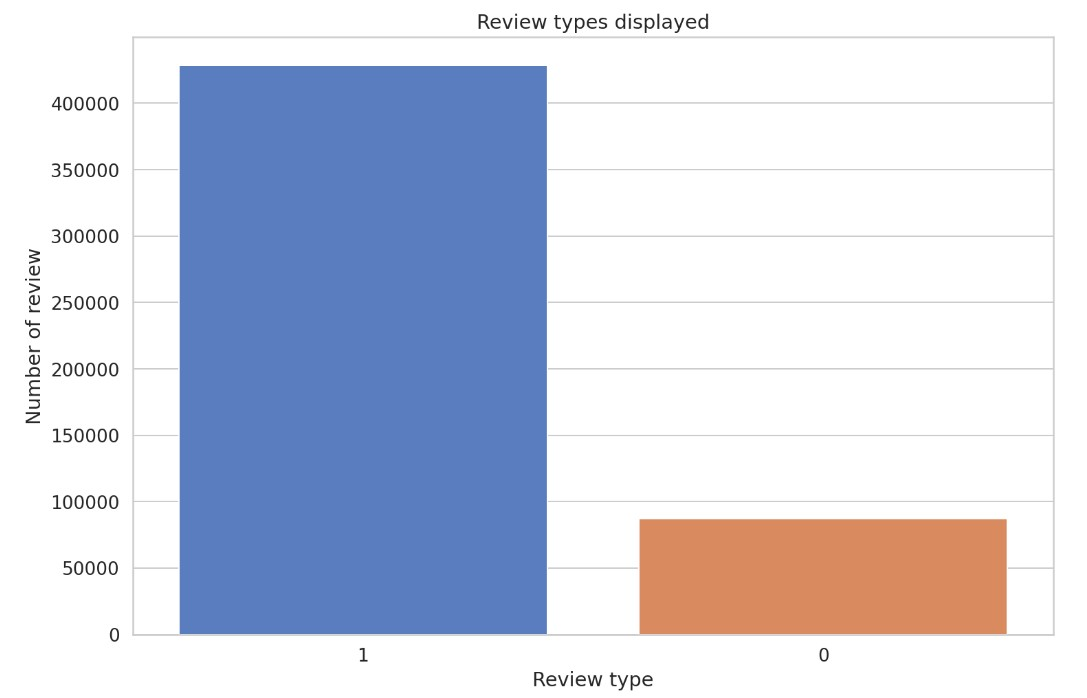
\includegraphics[width=1\textwidth]{images/rev1div.jpg}
\caption{Number of ratings per category}
\label{fig:fig_03}
\end{figure}
\FloatBarrier
\newpage
\subsubsection{Resample reviews}
In order to be able to train my model later on, I need to have the same amount of test data for each category. For this reason I should limit the larger category to the value of the smaller one. By doing so, the data will have  the same number of entries as in the figure~\ref{fig:fig_04}.

\begin{figure}[H]
\centering
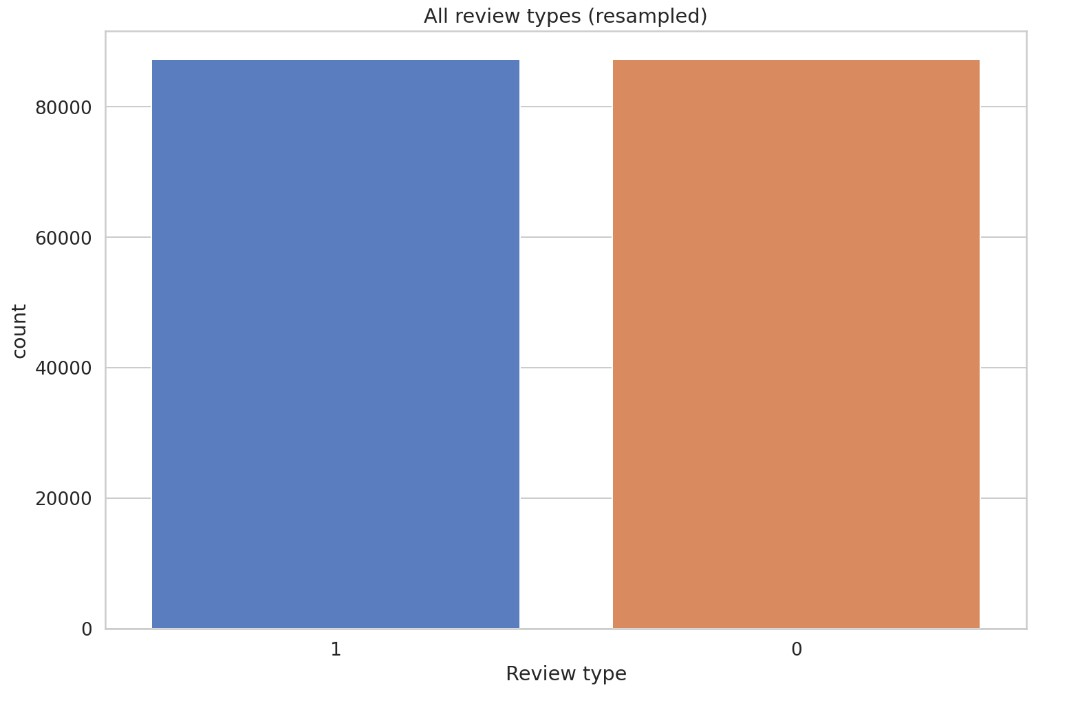
\includegraphics[width=1\textwidth]{images/rev2div.jpg}
\caption{Uniform size of the categories}
\label{fig:fig_04}
\end{figure}
\FloatBarrier

\subsubsection{Preprocessing}
In this section I deal with the preparation of the data to give then to the model.
The first thing to do is to split the dataframes I got after cleaning into 3 parts:
\begin{itemize}
    \item train set
    \item validation set
    \item test set
\end{itemize}

Training set is a sample of data used to fit the model, the model trains and learns from this data.\\
Validation set is used to evaluate the trained model. With the evaluation of the model it is possible to make a fine-tune of the model and to modify the hyperparameters.\\
Test set provides the gold standard used to evaluate the model.\\
\newpage
This is an example of a split\footnote{Reference figure \url{https://towardsdatascience.com/train-validation-and-test-sets-72cb40cba9e7}}: 
\begin{figure}[H]
\centering
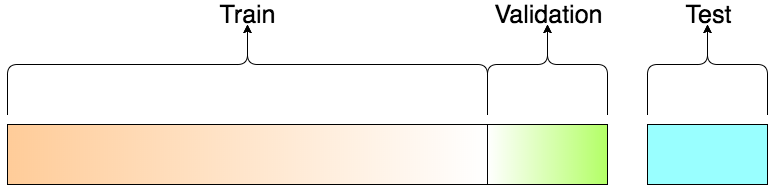
\includegraphics[width=1\textwidth]{images/traintestvali.jpg}
\caption{Data split}
\label{fig:fig_05}
\end{figure}
\FloatBarrier

Thanks to the library sklearn.model\_selection.train\_test\_split I can easily split my dataset in training and validation. As you can see in the figure~\ref{fig:fig_06} the division is done with a ratio 80\%(training)/20\%(validation)

\begin{figure}[H]
\centering
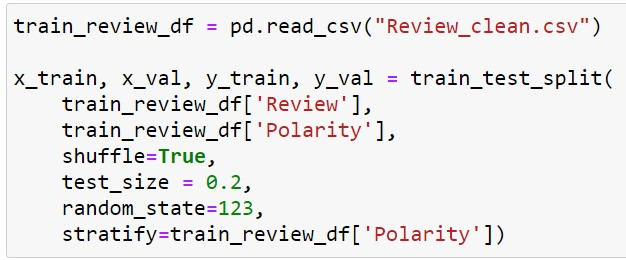
\includegraphics[width=0.7\textwidth]{images/traintest.jpg}
\caption{Sklearn method}
\label{fig:fig_06}
\end{figure}
\FloatBarrier

Now comes the central part of preprocessing for this dataset, to do this I used ktrain that allows me to convert the text of the reviews in features to give to the model.
The advantage is that I don't have to do every single preprocessing step manually, and all the steps are followed by the library itself.
To do this then I will use the texts\_from\_df function as shown in the figure~\ref{fig:fig_07}, so that I can use the previously created dataframe.

\begin{figure}[H]
\centering
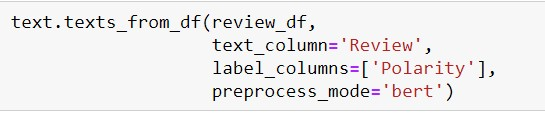
\includegraphics[width=0.7\textwidth]{images/preprocktrain.jpg}
\caption{Ktrain preprocessing}
\label{fig:fig_07}
\end{figure}
\FloatBarrier
\newpage
As you can see in the figure ~\ref{fig:fig_08}, the function will take as feature the column "Review" and as target "Polarity", it will also automatically download an already pretrained BERT model with its vocabulary.
The data for the BERT model has to be preprocessed in a certain way, so I have to indicate this at the preprocess\_mode line.

\begin{figure}[H]
\centering
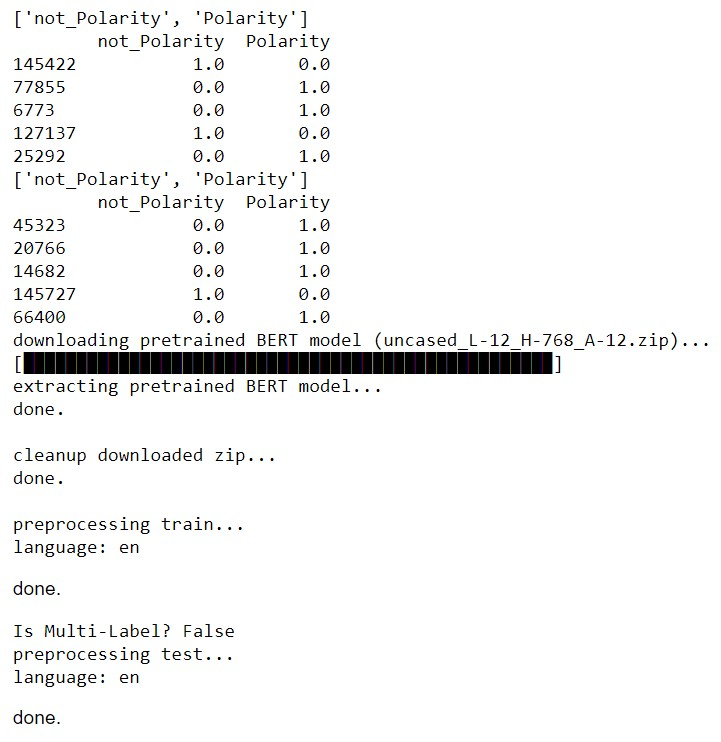
\includegraphics[width=0.8\textwidth]{images/preprocktrain2.jpg}
\caption{Ktrain preprocessing}
\label{fig:fig_08}
\end{figure}
\FloatBarrier

\newpage
\subsection{IMDB Review Dataset}

\subsubsection*{Dataframe structure}
In the image below you can see the structure of the dataset:
\begin{figure}[ht!]
\centering
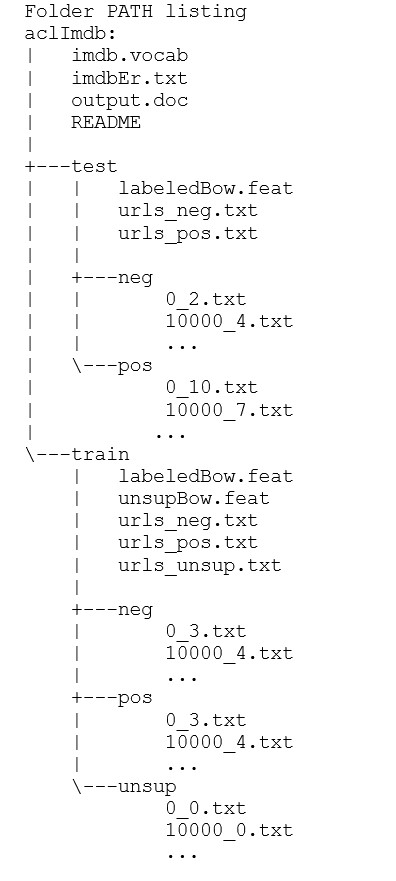
\includegraphics[width=0.5\textwidth]{images/foldertree.jpg}
\caption{Folder tree}
\label{fig:fig_0}
\end{figure}
\FloatBarrier

\subsubsection{Preprocessing}
Rispetto all'altro ds non ho bisgono di dover fare lavorazioni di pulizia o sui dati, ho solo tolto le cartelle che non erano inerenti al progetto, cosi come i dati non labellati.

We will now use the text\_dataset\_from\_directory utiliy to create a labeled dataset.

tf.data is a tensorflow API that allows you to create complex input pipelines from simple pieces, and reuse them.

To be able to work we need to divide the dataset in test and traning, in the case of IMDb we don't need to do that because it has already been divided as we have seen in the folder structure. What is missing, however, is a validation set, so I create a validation set using an 80/20 separation on the training data. To do this we will use tensorflow and keras, and for the validation set we are going to change the value of the validation\_split:

\begin{figure}[ht!]
\centering
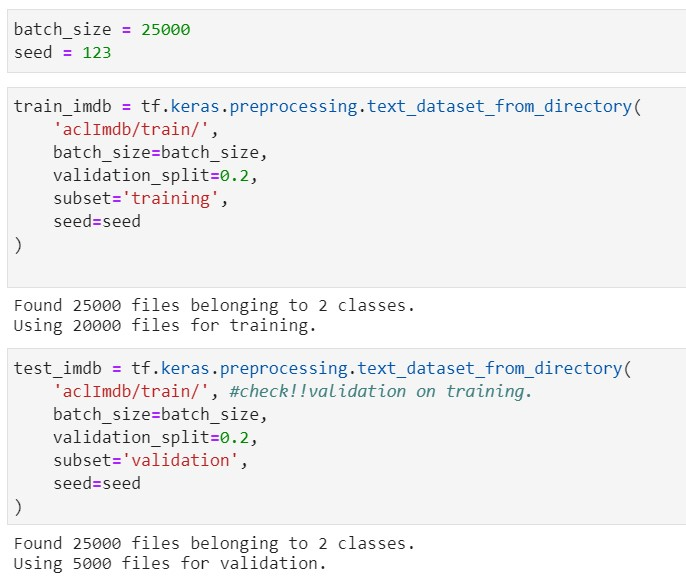
\includegraphics[width=1\textwidth]{images/preproimdb.jpg}
\caption{IMDb preprocessing}
\label{fig:fig_068}
\end{figure}
\FloatBarrier